\documentclass[12pt, a4paper]{article}
\usepackage{graphicx}
\usepackage[export]{adjustbox}
\usepackage{amsmath}
\graphicspath{{images/}}
\usepackage{titling}
\usepackage{subcaption}
\renewcommand\maketitlehooka{\null\mbox{}\vfill}
\renewcommand\maketitlehookd{\vfill\null}
\hbadness=10000

\title{Analysis of Adjacency Matrices by Spectral Graph Theory}
\author{
  Venkata Renu Jeevesh Madala\\
  2022102009
  \and
  Saumya Balina \\
  2022102069
  \and
  Moida Praneeth Jain \\
  2022101093
  \and
  Shreyas Badami \\
  2021113003
}
\date{MONSOON SEMESTER 2023}
\begin{document}
    \begin{titlepage}
      \maketitle
      \thispagestyle{empty}
    \end{titlepage}

    \section{Objective}
    % \begin{flushleft}
    The adjacency matrix provides a concise representation of the connections between nodes in a graph, while eigenvalues reveal important properties about
    the graph’s structure. Through analysis and computation of eigenvalues, this
    project aims to gain insights into the characteristics and behavior of graph networks, such as centrality measures, connectivity, and clustering.

      In a recent paper by Miller J. \cite{Jason}, methods to calculate the number of paths of length $k$ between any two vertices of a graph have been explored in great depth. These methods include calculating the eigenvalues of the graph's adjacency matrix and using them to formulate the number of paths. In this project, we aim to implement these methods and analyze them by comparing them against the usual method of matrix multiplication.

      In the paper on Graph Attention Networks published at ICLR 2018 \cite{GraphAttention}, graph attention networks (GATs), novel neural network architectures that operate on graph-structured data are discussed, leveraging masked self-attentional layers to address the shortcomings of prior methods based on graph convolutions or their approximations. They addressed several key challenges of spectral-based graph neural networks simultaneously, and make their model readily applicable to inductive as well as transductive problems. The graph attentional layer utilized throughout these networks is computationally efficient, allows for (implicitly) assigning different importances to different nodes within a neighborhood while dealing with different sized neighborhoods, and does not depend on knowing the entire graph structure upfront—thus addressing many of the theoretical issues with previous spectral-based approaches. Their models have successfully achieved or matched state-of-the-art performance across four well-established node classification benchmarks, both transductive and inductive. One potential improvement to graph attention networks is be able to handle larger batch sizes.
    % \end{flushleft}
    \section{Introduction}

      \subsection{Eigenvalue and Eigenvector}
      \begin{flushleft}
      For a matrix $A$, a vector which when multiplied by $A$ gives a scalar multiple of itself is called an eigenvector of $A$. This scalar multiple is called the corresponding eigenvalue.

      $$Ax = \lambda x$$

      $x$ is an eigenvector and $\lambda$ is the corresponding eigenvalue

      \end{flushleft}
      \subsection{Graph}
      A graph is a set of vertices $V$ connected by a set of edges $E$.  
      $$G = (V, E)$$
        \subsubsection{Directed Graph}
        A directed graph is a graph where each edge represents an ordered pair of vertices. In-degree of a vertex is the number of edges directed towards the vertex. Out-degree of a vertex is the number of edges directed from the vertex.
        \subsubsection{Undirected Graph}
        An undirected graph is a graph where each edge represents an unordered pair of vertices. Degree of a vertex is the number of edges the vertex is connected to.

        \subsubsection{Path}
        \begin{flushleft}
        A sequence of vertices $$V_1V_2V_3...V_n$$ is a path if 
        $$\forall i \in \{1,2,3,..,n-1\} \qquad (V_{i}, V_{i+1}) \in E$$

        The length of such a path is $n-1$
        \end{flushleft}

      \subsection{Adjacency Matrix of a graph}
      For a graph $G$ with $n$ vertices, its adjacency matrix $A(G)$ is an $n$ by $n$ square matrix with $a_{i,j}$ equal to the number of edges connecting $V_i$ to $V_j$

        \subsubsection{Properties}
        For an undirected graph $G$
        \begin{itemize}
          \item $A(G)$ is symmetric 
          \item $A(G)$ has real eigenvalues
          \item $(i,j)$ entry of $A(G)^k$ represents the number of paths of length k from $V_i$ to $V_j$ $\quad \forall k \ge 1$
        \end{itemize}

    \section{Centrality Measures}
    Centrality measures use graph theory to calculate the importance of any given node in a network. Centrality has different types and each type or metric defines the “importance” of a node from different perspectives and further provides relevant analytical information about the graph and its nodes.\cite{Disney22}
    \subsection{Eigen Centrality}
    \begin{flushleft}

    Eigen Centrality measures the importance of a node in a graph as a function of the importance of its neighbours. If a node is connected to highly important nodes, it will have a higher Eigen Vector Centrality score as compared to a node which is connected to lesser important nodes.
    
    Eigen Centrality measures a node’s influence by also taking into account how well connected a node is, how many links their connections have, and so on through the network.
    
    By calculating the extended connections of a node, Eigen Centrality can identify nodes with influence over the whole network, not just those directly connected to it.

    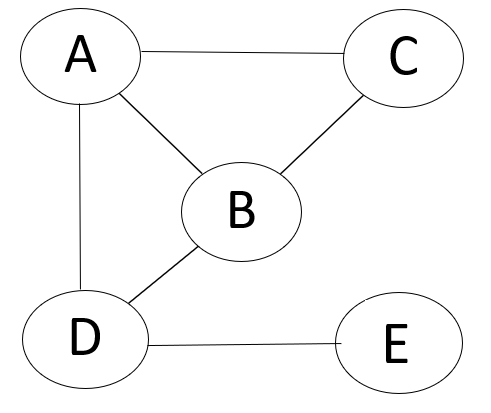
\includegraphics[width=0.5\textwidth, center]{graph}
    
    The adjacency matrix A of the above graph will be as shown below:
    \begin{equation*}
    \begin{bmatrix}
    - & 1 & 1 & 1 & 0 \\
    1 & - & 1 & 1 & 0 \\
    1 & 1 & - & 0 & 0 \\
    1 & 1 & 0 & - & 1 \\
    0 & 0 & 0 & 1 & - \\
    \end{bmatrix}
    \end{equation*}
    
    Let’s assume that in the above graph, the importance of each node is measured by its degree, such that the higher the degree of a node, the more important it is in the graph. Degrees of various nodes are shown below:
    
    \begin{table}[h]
    \centering
    \begin{tabular}{|c|c|}
    \hline
    Node & Degree \\
    \hline
    A & 3 \\
    B & 3 \\
    C & 2 \\ 
    D & 3 \\
    E & 1 \\
    \hline
    \end{tabular}
    \end{table}
    
    The above can also be represented as a vector V as shown below:

    \begin{equation*}
    \begin{bmatrix}
    3 \\
    3 \\
    2 \\
    3 \\
    1 \\
    \end{bmatrix}
    \end{equation*}

    Mathematically the Eigen Vector Centrality is calculated as below:

    \begin{equation*}
    \begin{split}
        A \times V & = \begin{bmatrix}
    - & 1 & 1 & 1 & 0 \\
    1 & - & 1 & 1 & 0 \\
    1 & 1 & - & 0 & 0 \\
    1 & 1 & 0 & - & 1 \\
    0 & 0 & 0 & 1 & - \\
    \end{bmatrix} 
    \begin{bmatrix}
    3 \\
    3 \\
    2 \\
    3 \\
    1 \\
    \end{bmatrix} \\ 
    & = \begin{bmatrix}
    0\times3 + 1\times3 + 1\times2 + 1\times3 + 0\times1 \\
    1\times3 + 0\times3 + 1\times2 + 1\times3 + 0\times1 \\
    1\times3 + 1\times3 + 0\times2 + 0\times3 + 0\times1 \\
    1\times3 + 1\times3 + 0\times2 + 0\times3 + 1\times1 \\
    0\times3 + 0\times3 + 0\times2 + 1\times3 + 0\times1 \\
    \end{bmatrix} \\
    \Rightarrow A \times V & =
    \begin{bmatrix}
    8 \\
    8 \\
    6 \\
    7 \\
    3 \\
    \end{bmatrix}
    \end{split} 
    \end{equation*}

    The resultant 1-D vector in the above equation gives the Eigen Vector Centrality (EVC) score for each of the nodes in the graph.

    The effect of the first iteration of multiplication can be visualized as shown below:

    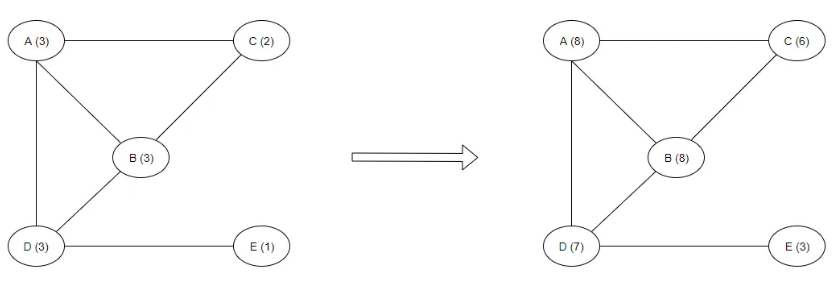
\includegraphics[width=0.9\textwidth,center]{Transform}

    As you can see above, nodes A and B both have a high score of 8 since both of them are connected to multiple nodes with high degrees (importance) while node E has a score of 3 since it is only connected to a single node of degree 3.
    
    Observe that the EVC score value for each node in the resultant vector is nothing but the sum of degrees of its neighbouring nodes.
    
    Multiplying the resultant vector again with the adjacency matrix of the graph helps the EVC score spread out in the graph to get a more globally prominent EVC score vs a localized EVC score for each node in the graph. After the first iteration of multiplication, each node’s EVC score is a function of only its direct (first degree) neighbours, thus is a localized score which might not be accurate at a global level in the graph.

    Thus, the following observations can be made:

    \begin{enumerate}
    \item After the first iteration of multiplication, each node gets its EVC score from its direct(first degree) neighbours.
    
    \item In the second iteration, when we multiply the resultant vector again with the adjacency matrix, each node again gets its EVC score from its direct neighbours but the difference in the second iteration is that this time, the scores of the direct neighbours have already been impacted by their own direct(1st degree) neighbours previously(from the first iteration of multiplication) which eventually helps the EVC score of any node to be a function of its 2nd degree neighbouring nodes as well.
    
    \item In subsequent iterations of multiplication, the EVC score of graph nodes keeps getting updated by getting impacted by EVC scores from neighbouring nodes of farther degrees (3rd, 4th and so on).
    
    \end{enumerate}
    Repeated multiplication makes the EVC score of every node eventually be a function of or dependent on several degrees of its neighbouring nodes, thereby providing a globally accurate EVC score for each node. Usually, the process of multiplying the EVC vector with the adjacency matrix is repeated until the EVC values for nodes in the graph reach an equilibrium or stop showing the appreciable change.

    One sample application of EVC is the calculation of Page Rank or Page Rank algorithm used by Google and many other companies to rank web pages on the internet by relevance. Page Rank is a direct variant of EVC. Web pages on the World Wide Web have links that point to/from other web pages. You can think of each web page as a node in the graph and each outgoing/incoming link as a directed edge leading to/from another web page on the web, thereby making up the whole World Wide Web graph. The graph of web pages in the world wide web undergoes several iterations of EVS calculation so as to calculate globally accurate relevance rankings of each web page. The web pages with high EVC scores can then be targeted for marketing and other commercial purposes. \cite{Bhasin22}

  \end{flushleft}
    \section{Clustering}
    \begin{flushleft}
        Graph clustering, also known as community detection, is the process of partitioning a graph into groups or clusters, where nodes within the same cluster are more closely connected to each other than to nodes in other clusters. The goal of graph clustering is to uncover meaningful structures or communities within a graph, allowing us to better understand the relationships and organization of the nodes. Clustering algorithms aim to maximize intra-cluster connectivity while minimizing inter-cluster connectivity, resulting in groups of nodes that are densely connected internally and sparsely connected externally.
        
        
        \subsection{Some popular methods of graph clustering}
        Several algorithms exist for graph clustering, each with its own approach and assumptions.
        \subsubsection{K-Means Graph Clustering Method}
        \begin{flushleft}
            This method partitions the graph into clusters that appear with a k-shape. It uses k-means to compute the centroids and their vector quantities. The steps involved in constructing the K-means clustering method include: selecting K to represent the original centroids, assigning points to the nearest centroids from the K-cluster, and conducting a re-evaluation of the centroids to ensure they do not change. One advantage of this method is that it can handle large data sets.

            \begin{figure}[h]
            \centering
            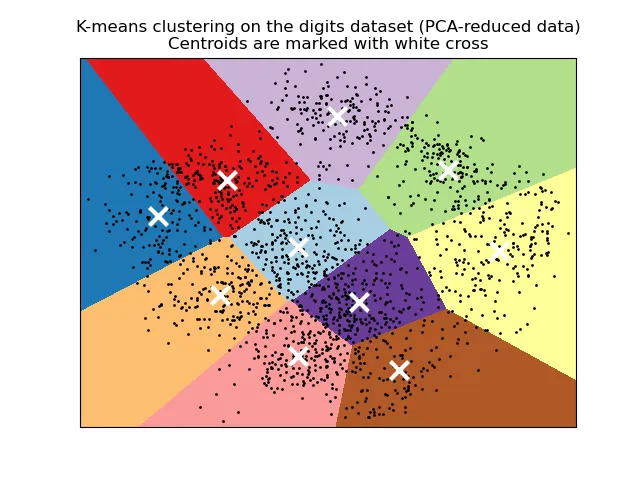
\includegraphics[width=0.5\textwidth]{k-means_based.png}
            \end{figure}
        \end{flushleft}

        \subsubsection{Spectral clustering}
        \begin{flushleft}
            This approach leverages the spectral properties of the graph to perform clustering. It involves transforming the graph into a matrix representation and using eigenvalue decomposition or other spectral techniques to extract clusters. Spectral clustering can handle graphs with irregular structures and is particularly effective for identifying clusters with non-convex shapes.
            \begin{figure}[h]
            \centering
            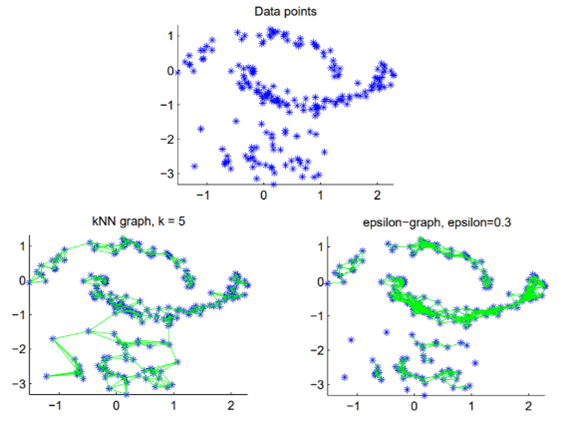
\includegraphics[width=0.5\textwidth]{spectral_based.png}
            \end{figure}
        \end{flushleft}

        \subsubsection*{}
        \begin{flushleft}
        The choice of clustering algorithm depends on various factors, such as the nature of the graph, the size of the graph, the desired level of granularity, and the specific goals of the analysis. Additionally, it is important to consider the scalability and computational complexity of the algorithm, as some methods may be more suitable for large-scale graphs. Once the graph clustering algorithm has been applied, the resulting clusters can be analyzed to gain insights into the structure and organization of the graph. Cluster evaluation measures, such as modularity, silhouette coefficient, or normalized mutual information, can be used to assess the quality of the clustering results.
        \end{flushleft} 

        \subsection{Connection between Clustering and Eigenvalues}

        \subsubsection{Spectral Radius}
        \begin{flushleft}
        One important eigenvalue associated with the adjacency matrix is the spectral radius, which is the largest eigenvalue of the matrix.
        
        The spectral radius provides information about the expansion properties of the graph. If the spectral radius is small, it suggests that the graph has a well-connected structure with tight clusters. On the other hand, a large spectral radius indicates a more dispersed and less clustered graph.
        \end{flushleft}

        \subsubsection{Algebraic Connectivity}
        \begin{flushleft}
        Another relevant eigenvalue is the second smallest eigenvalue, also known as the algebraic connectivity.
            
        The algebraic connectivity measures the connectivity and robustness of the graph. Larger algebraic connectivity implies that the graph has more connections between its nodes, indicating a higher likelihood of clustering.
        \end{flushleft}
        \subsubsection*{}
        \begin{flushleft}
        Additionally, the eigenvalues of the adjacency matrix can be used to identify the number of clusters in a graph. This is achieved by examining the gaps between consecutive eigenvalues. Large gaps suggest the presence of distinct clusters, while small gaps indicate a more homogeneous graph without well-defined clusters.

        Furthermore, eigenvectors associated with the eigenvalues can provide information about the clustering structure within the graph. The eigenvectors are vectors that correspond to the eigenvalues and represent the distribution of nodes within the graph. By examining the components of the eigenvectors, it is possible to identify nodes that belong to the same cluster or community.
        \end{flushleft}

        \subsection{Clustering with Linear Algebra}
        \begin{flushleft}
        \subsubsection{Creating a Dataset}
        \begin{flushleft}
        Our data consists of 200 2-vectors simulated by the \texttt{make\_blobs} function in scikit-learn.

        \begin{figure}[h]
        \centering
        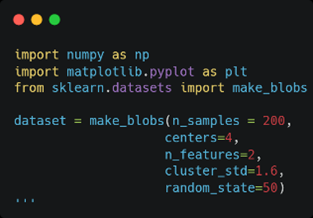
\includegraphics[width=0.5\textwidth]{data_create.png}
        \end{figure}
        Plotting them, we see we see our data spanning following 2D-space.
        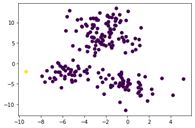
\includegraphics[width=0.5\textwidth,center]{data_rep.png}
        \end{flushleft}
        \subsubsection{Clustering Analysis}
        \begin{flushleft}
        Let's analyze the data using a clustering method. We start by specifying a cluster assignment vector $c$, which informs us about which vector belongs to which cluster. 

        For this example, we arbitrarily initiate the cluster assignments as $c = [1,2,3,1,2,3,1,2,3]$, indicating that cluster 1 contains vectors $v_1$, $v_4$, $v_7$, cluster 2 contains vectors $v_2$, $v_5$, $v_8$, and cluster 3 contains vectors $v_3$, $v_6$, $v_9$.
        \end{flushleft}
        \begin{enumerate}
        \item\textbf{Centroid Calculation}
        \begin{flushleft}
        To calculate the similarity of the data points to each other, we use a group representative called the centroid. The centroid for each cluster is calculated as follows:

        \[
        \text{{centroid}}_j = \frac{1}{{|G_j|}} \sum_{i \in G_j} x_i
        \]

        where $G_j$ represents the elements in group $j$, and $x_i$ denotes the vectors in the dataset.
        \end{flushleft}

        \item\textbf{Clustering Quality}
        \begin{flushleft}
            We can assess the quality of the current clustering assignment by calculating the mean square distance from the vectors to their associated centroids. This is done using the following equation:

            \[
            \mathbf{z}_1 = \frac{1}{|G_1|} \sum_{i \in G_1} \mathbf{x}_i
            \]

            Now we have every ingredient needed to calculate the quality of the current clustering assignment. For this, we calculate the mean square distance from the vectors to their associated representatives with the following equation:

            \[
            \text{Quality} = \frac{1}{N} \sum_{i=1}^{N} \|\mathbf{x}_i - \mathbf{z}_{c_i}\|^2
            \]

            where $N$ is the total number of vectors, $x_i$ represents the vectors, and $z_{c_i}$ denotes the centroid corresponding to the cluster assignment $c_i$.

            \begin{figure}[h]
            \centering
            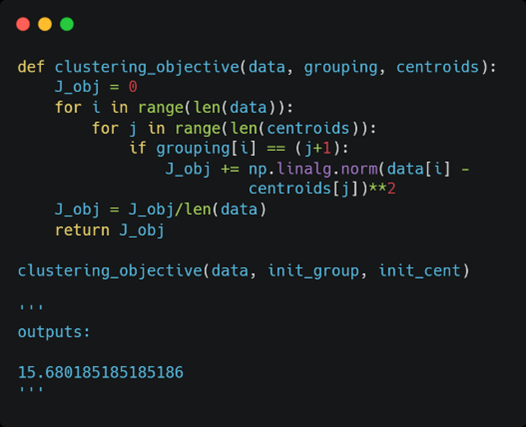
\includegraphics[width=0.5\textwidth]{root_mean_calc.png}
            \end{figure}
           
        \end{flushleft}
        \end{enumerate} 

        \subsection{Visual Application}
        \begin{flushleft}
                With the initial dataset we have a high loss (mean-squared error):
                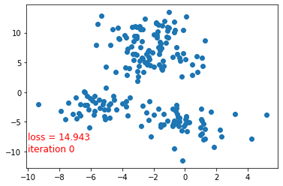
\includegraphics[width=0.5\textwidth,center]{example1.png}
            \begin{enumerate}
                \item In Step 1 we assign the data points to the cluster with the nearest centroid:
                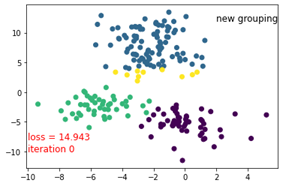
\includegraphics[width=0.5\textwidth,center]{images/example2.png}
                
                \item In Step 2 we calculate the centroids again with the assigned data points:
                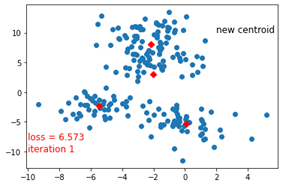
\includegraphics[width=0.5\textwidth,center]{example3.png}

                \item Our final clustering solution then looks like this:
                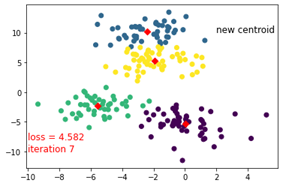
\includegraphics[width=0.5\textwidth,center]{example5.png}

            \end{enumerate}
                In this example, linear algebra techniques were used to perform clustering analysis. The centroids obtained from the clustering process can be used as representatives of the clusters, providing valuable insights into the dataset.
            
        \end{flushleft}
        \end{flushleft}
    \end{flushleft}
  
    \section{Connectivity}
    We will analyse the connectivity of a graph using its adjacency matrix and its eigenvalues.

    \subsection{Connected Components \cite{baeldung}}
    \begin{flushleft}
    Consider a regular undirected graph $G$ (each vertex having degree $d$), and some eigenvector $x$ of $A(G)$ with its corresponding eigenvalue $\lambda$

    $$A(G)*x = \lambda*x$$
    $$\lambda x_i = \sum_{j} A_{ij}x_j$$
    $$|\lambda||x_i| \le \sum_{j} |A_{ij}||x_i|$$
    $$ |\lambda||x_i| \le d|x_i| \qquad (Since \quad |x_j| \le |x_i| \forall j)$$
    $$|\lambda| \le d$$

    All the eigenvalues of this graph are smaller than or equal to $d$. \cite{bhaskara4}

    Upon setting all $x_i$ to 1, we get $Ax = dx$, which gives
    $$\lambda_{max} = d$$

      The multiplicity of the maximum eigenvalue (equal to $d$) gives the number of connected components of $G$. \cite{bhaskara5} The number of connected components of a graph have various applications in different fields

      \begin{itemize}
        \item Social Network Analysis: Connected components are used to identify a set of individuals as a community. By finding these components, insights on information flow and social interactions are studied by researchers.
        \item Image Processing: Segmentation of objects and finding regions of interest is done by finding the connected components of an image. The image is converted into a graph, and then pixels sharing similar characteristics are grouped together. This is useful for object recognition and feature extraction.

        \item Network Routing: In large-scale computer networks, connected components are used by routing algorithms to determine the best path that the data packets should take in order to reach their destination.
      \end{itemize}
    \end{flushleft}

    \subsection{Number of paths in a graph \cite{mitpaths}}
    \begin{flushleft}
    Consider an undirected graph $G$ with adjacency matrix $A(G)$. Let $\lambda_1,\lambda_2,\lambda_3,...,\lambda_n$ be the eigenvalues of $A(G)$
      $$\forall i,j \quad \exists c_1,c_2,c_3,...,c_n \quad (A(G)^k)_{ij} = c_1\lambda_1^k + c_2\lambda_2^k + c_3\lambda_3^k + ... + c_n\lambda_n^k \quad \forall k \ge 1$$
      For each index $(i, j)$, upon identifying its corresponding $c_i$ values, the number of paths from $V_i$ to $V_j$ of any length can be calculated in constant time using this equation.

      Similarly, the total number of self loops of length k is given by
      $$\lambda_1^k + \lambda_2^k + \lambda_3^k + ... + \lambda_n^k$$


      Since the number of paths of length $k$ between two vertices $V_i$ and $V_j$ is given by $(A(G)^k)_{i,j}$, for a given $(i,j)$ \\ we precalculate $(A(G)^k)_{i,j} \quad \forall k \in \{1,2,...,n\}$ and store them in the matrix
    \begin{equation*}
      Y = 
    \begin{bmatrix}
    (A(G))_{i,j} \\
    (A(G)^2)_{i,j} \\
    (A(G)^2)_{i,j} \\
    (A(G)^3)_{i,j} \\
    . \\
    . \\
    . \\
    (A(G)^{n})_{i,j} \\
    \end{bmatrix}
    \end{equation*}

    Now, after calculating the eigenvalues of the adjacency matrix $A(G)$, we construct the followng matrix
 \begin{equation*}
      A = 
    \begin{bmatrix}
      \lambda_1 & \lambda_2 & \lambda_3 & . & . & . & \lambda_n\\
      \lambda^2_1 & \lambda^2_2 & \lambda^2_3 & . & . & . & \lambda^2_n\\
      \lambda^3_1 & \lambda^3_2 & \lambda^3_3 & . & . & . & \lambda^3_n\\
      . & . & . & . & . & . & . \\
      . & . & . & . & . & . & . \\
      . & . & . & . & . & . & . \\
      \lambda^n_1 & \lambda^n_2 & \lambda^n_3 & . & . & . & \lambda^n_n\\
    \end{bmatrix}
    \end{equation*}

    To solve for the values of $c_i$, we solve the system of linear equations
      $$A*C=Y$$
      After we get the resultant $C$ vector, we can compute the number of paths of length $k \quad \forall k \ge 1$ simply be performing the dot product
      \begin{equation*}
        \begin{bmatrix}
        c_1 \\
        c_2 \\
        c_3 \\
        . \\
        . \\
        . \\
        c_n \\
        \end{bmatrix}
        .
        \begin{bmatrix}
        \lambda_1^k \\
        \lambda_2^k \\
        \lambda_3^k \\
        . \\
        . \\
        . \\
        \lambda_n^k \\
        \end{bmatrix}
      \end{equation*}

    Since we only have to precompute the $c_i$ values by solving linear equation in $n$ variables, we can find number of paths of length k between two vertices for any arbitrarily large k in a fraction of the time required by regular matrix multiplication. 

    \begin{figure}
      \centering
      \begin{subfigure}{0.49\textwidth}
        \centering
    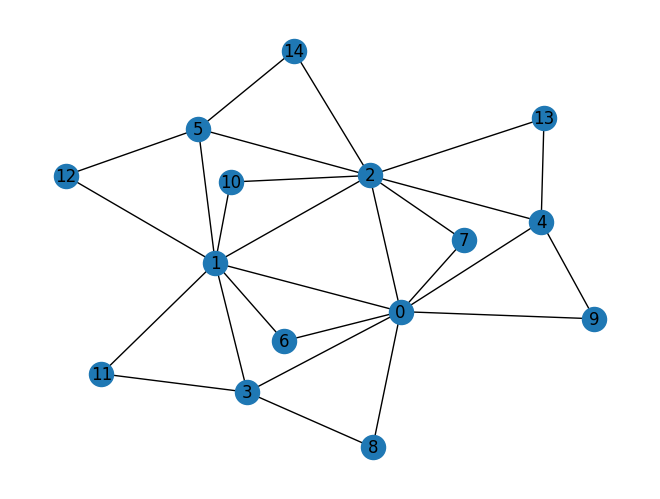
\includegraphics[width=1\textwidth]{15nodesgraph}
      \end{subfigure}
      \begin{subfigure}{0.49\textwidth}
        \centering
    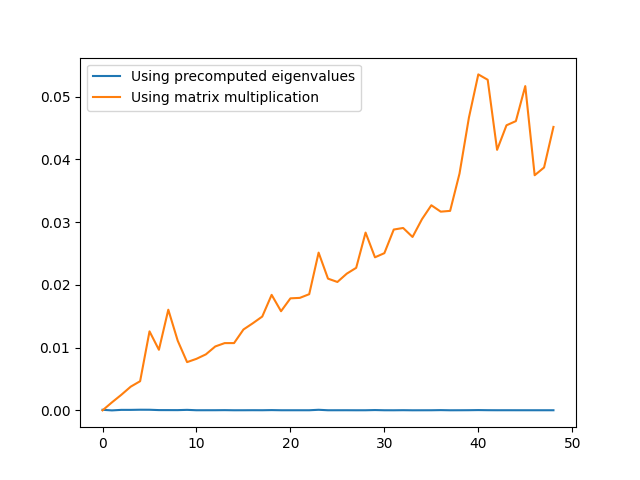
\includegraphics[width=1\textwidth]{15nodesoutput}
      \end{subfigure}
    \caption{Comparison in speed for a graph with 15 nodes}
    \end{figure}

    \begin{figure}
      \centering
      \begin{subfigure}{0.49\textwidth}
        \centering
    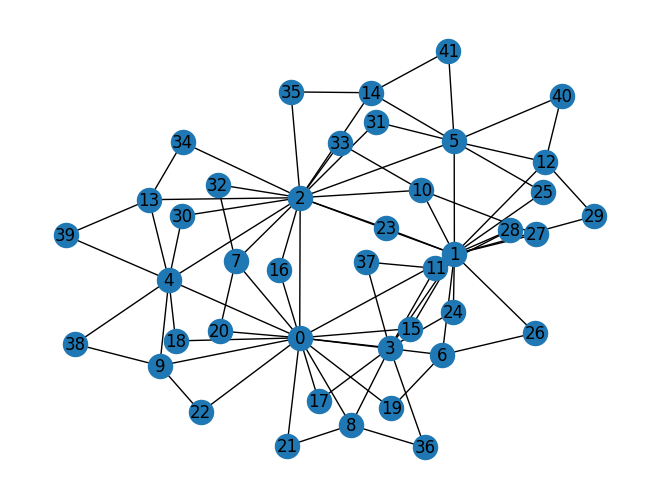
\includegraphics[width=1\textwidth]{42nodesgraph}
      \end{subfigure}
      \begin{subfigure}{0.49\textwidth}
        \centering
    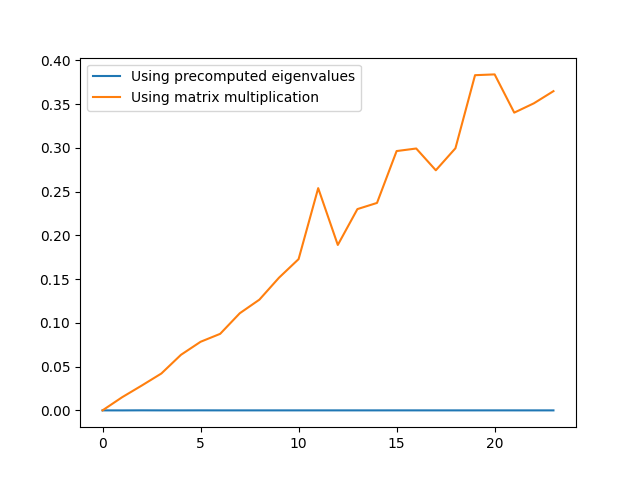
\includegraphics[width=1\textwidth]{42nodesoutput}
      \end{subfigure}
    \caption{Comparison in speed for a graph with 42 nodes}
    \end{figure}
      The number of paths of given length between any two vertices is a very useful metric to have
      \begin{itemize}
        \item Network Analysis: The number of paths between any two access points in a network informs us of its reliability. We can figure out the number of alternate paths the network can take, and how to distribute the packets between all the paths in order to optimally transmit data.

        \item Reachability Analysis: The presence of a direct or indirect path between any two vertices gives insights on information flow and communication possibilities. The number of paths tells us how easily accessible any vertex is from any other vertex.

        \item Disease Spread: While modelling the spread of a disease, individuals and locations act as vertices in the graph, and the number of paths quantify how likely it is that the disease spread to the other end of that path. This informs us regarding control strategies and which locations require quarantine measures the most.
      \end{itemize}

    \end{flushleft} 

    \section{Conculsion}
    \begin{flushleft}
      We have successfully implemented the methods to calculate number of paths and shown that they are significantly faster than conventional methods, given a certain amount of precomputation.
    \end{flushleft}

    \begin{thebibliography}{9}
    \bibitem{baeldung}
    Science, B. O. C., Science, B. O. C. (2022). Connected Components in a Graph | Baeldung on Computer Science. Baeldung on Computer Science. https://www.baeldung.com/cs/graph-connected-components
    \bibitem{bhaskara4}
    Aditya Bhaskara, CS Utah (2016). Graph Partitioning, basic linear algebra https://users.cs.utah.edu/~bhaskara/courses/x968/notes/lec4.pdf
    \bibitem{bhaskara5}
    Aditya Bhaskara, CS Utah (2016). Eigenvalues of $A_G$ and the Laplacion https://users.cs.utah.edu/~bhaskara/courses/x968/notes/lec5.pdf

    \bibitem{mitpaths}
    Derek Chen, Advay Goel (2021). Spectral Graph Theory https://math.mit.edu/research/highschool/primes/materials/2021/\\December/Chen-Goel.pdf

    \bibitem{Bhasin22}
    Bhasin, J. (2022, March 30). Graph Analytics — Introduction and Concepts of Centrality. Medium. https://towardsdatascience.com/graph-analytics-introduction-and-concepts-of-centrality-8f5543b55de3

    \bibitem{Disney22}
    Disney, A. (2022, October 27). Social network analysis: Understanding centrality measures. Cambridge Intelligence. https://cambridge-intelligence.com/keylines-faqs-social-network-analysis/

    \bibitem{Tuzsus22}
    Tuzsus, D. (2022, May 14). Introduction to Applied Linear Algebra: K-Means Clustering. Medium. https://medium.com/mlearning-ai/introduction-to-applied-linear-algebra-k-means-clustering-c6885cad0f7f
    \bibitem{Wong23}
    Wong, K. J. (2023, May 27). 6 Types of Clustering Methods — An Overview - Towards Data Science. Medium. https://towardsdatascience.com/6-types-of-clustering-methods-an-overview-7522dba026ca

    \bibitem{Jason}
    Miller, J. (2020, June 8). An Introduction to Spectral Graph Theory https://sites.math.washington.edu/\~morrow/336\_20/papers20/jason.pdf

  \bibitem{GraphAttention}
Veličković, P., Cucurull, G., Casanova, A., Romero, A., Liò, P., \& Bengio, Y. (2018). Graph Attention Networks. arXiv (Cornell University). https://doi.org/10.17863/cam.48429
    \end{thebibliography}
\end{document}
